\chapter{Laboratórne overenie funkčnosti}

V tejto kapitole predstavíme vlastnosti nami skonštruovaného robota pri laboratórnych testoch. Zameriame sa prevažne na správanie sa robota v ovládanom režime, jeho schopnosť presúvať sa po šikmých plochách a jeho celkovú stabilitu vo vyšších rýchlostiach.

Pri režime statického balansovania na mieste sa zameriame na priemernú odchýlku od nulového náklonu, amplitúdu oscilácií, celkovú prejdenú vzdialenosť (so zaradením PIDu C aj bez neho), veľkosť prúdu vstupujúceho do H-mostíka vzhľadom na striedu a rýchlosť ustálenia robota po postrčení.

Všetky grafy použté v tekto kapitole boli vytvorené s použitím nami napísaného python programu a dáta v nich zobrazené boli získané prostredníctvom sériovej komunikácie medzi počítačom a robotom.  

\section{Základné parametre robota}
Vychádzajúc z modelu robota, ktorý sme vytvorili v kapitole \ref{ch:analyza} sme namerali tieto parametre robota:

\begin{multicols}{2}
\begin{itemize}
\item{$R = 7,2 ~\Omega$}
\item{$K_e = 0,334$}
\item{$K_m = 0,093$}
\item{$J_k = 1,598x10^{-3}~ kgm^{2}$}
\item{$J_s = 4,025x10^{-2}~ kgm^{2}$}
\item{$r = 3,4x10^{-2}~ m$}
\item{$m_k = 4,7x10^{-2}~ kg$ss}
\item{$m_p = 1,07 ~kg$}
\item{$L = 0,145 ~m$}
\end{itemize}
\end{multicols}

Pri meraní zotrvačnosti kolesa sme použili vzorec \ref{eq:J_wheel}:
\begin{equation}
J_k = m_kr^2
\label{eq:J_wheel}
\end{equation}

a pre zotrvačnosť celého robota:
\begin{equation}
J_s = \dfrac{m_pgLT^2}{4\pi^2}
\label{eq:J_robot}
\end{equation}
kde $T$ je perióda oscilácie robota okolo osi kolies po vychýlení o malý uhol.

S praktického uhla pohľadu je ďalšou dôležitou informáciou výdrž nami použitej batérie. Tá pri balansovaní na mieste vydržala pri počiatočnom plnom nabití pracovať takmer hodinu zatiaľ čo čas výdrže batérie v ovládači sa pohyboval na úrovni zhruba 20 hodín. Obe batérie sú nabíjateľné, pričom nabíjací cyklus trvá približne 4 hodiny v prípade batérie robota a asi 2 hodiny v prípade batérie ovládača Tab.~\ref{tab:battery_charge}. 
\bgroup
\def\arraystretch{1.5}
\begin{table}[h]
\centering
\begin{tabular}{|m{3cm}|c|c|}
\hline
 & \textbf{Výdrž [h]} & \textbf{Doba nabíjania [h]}\\
\hline
Batéria robot & $1$ & $4$\\
Batéria ovládač & $20$ & $2$\\
\hline
\end{tabular}
\caption{Charakteristiky batérií}
\label{tab:battery_charge}
\end{table}
\egroup

\section{Parametre robota pri balansovaní na mieste}
Pri balansovaní na mieste môže užívateľ zvolliť z dvoch režimov prevádzky. V prvom režime robot balansuje bez toho aby sa snažil udržať počiatočnú pozíciu, v druhom sleduje celkovú prejdenú vzdialenosť a snaží sa ju udržať na minime. Druhý stav je výhodný najmä v prípade ak sa robot nachádza na naklonenej plošine, kde mu sledovanie prejdenej vzdialenost umožnuje pridávať rýchlosť natoľko aby sa udržal v nehybonsti.

Testovanie správanai robota prebiehalo po pripojení k počítaču dlhým, flexibilnýcm káblom, ktorý nám umožnil komunikáciou cez sériovú linku zhromaždiť údaje o stave robota v jenotlivých časových okamihoch. Pomocu týchto dát boli následne vytvorené grafy zobrazené na  \figurename~\ref{fig:combination}. Na osi Y sa nachádzajú odchýlky od pravého uhla pre jednotlivé sledované vzorky. Čas medzi jednotlivými vzorkami bol $t_vz = 50ms$, čiže celkový časový interval, počas ktorého sme sledovali správanei robota trval 50 sekúnd.

Z porovnania grafov na \figurename~\ref{fig:combination} je zrejmé, že pri vypnutom sledovaní polohy bol robot schpný presnejšie regulovať uhlovú odchýlku od pravého uhla. Je zjavné, že v tomto režime odchýlka málokedy prekročila hodnotu 1°, čo sa nedá povedať o režime, v ktorom bolo toto sledovanie zapnuté. Nevýhodou ale bolo, že aj za relatívne krátky čas merania došlo k posunu robota o $10~cm$ oproti počiatočnej polohe, čo v prípade merania v druhom režime nebol problém. Pri sledovaní polohy vzdialenosť robota od počiatočnej polohy nikdy neprekročila $4cm$ pričom mal vždy robot tendenciu vracať sa do počiatočnej polohy a oscilovať okolo nej.
 

\begin{figure}[h!]
\centering
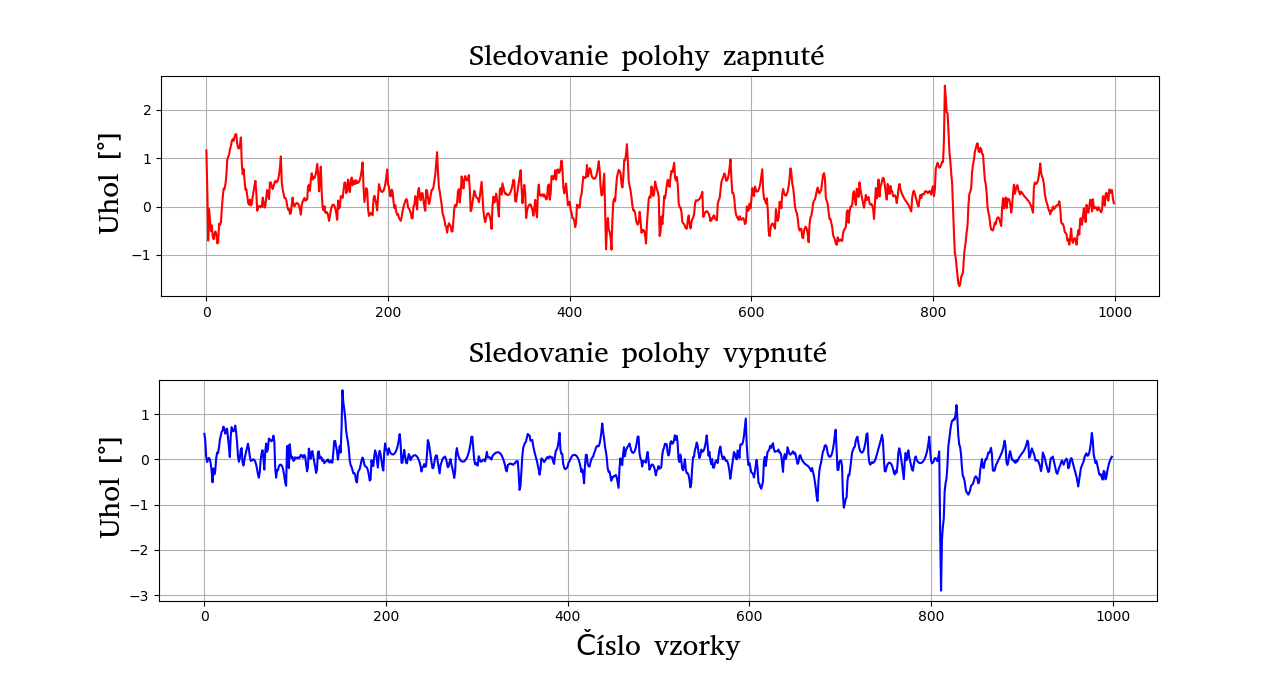
\includegraphics[width=16cm]{combination}
\label{fig:combination}
\caption{Náklon robota v čase}
\end{figure}   



\todo[inline]{graf, bez a s držaním, na rovine na svahu, spotreba pri týchto stavoch (dokončiť to snímanie prúdu!!!!)}

\section{Parametre robota pri ovládanom pohybe}
\todo[inline]{to isté ako pri (hore) + ovládanie zo strany na stranu, max. dosiahnutá rýchlosť}
